\documentclass[11pt,twoside,a4paper]{article}
% http://www-h.eng.cam.ac.uk/help/tpl/textprocessing/latex_maths+pix/node6.html symboles de math
% http://fr.wikibooks.org/wiki/Programmation_LaTeX Programmation latex (wikibook)
%=========================== En-Tete =================================
%--- Insertion de paquetages (optionnel) ---
\usepackage[english]{babel}   % pour dire que le texte est en fran{\'e}ais
\usepackage{a4}	             % pour la taille   
\usepackage[T1]{fontenc}     % pour les font postscript
\usepackage{epsfig}          % pour gerer les images
%\usepackage{psfig}
\usepackage{amsmath, amsthm} % tres bon mode mathematique
\usepackage{amsfonts,amssymb}% permet la definition des ensembles
\usepackage{float}           % pour le placement des figure
\usepackage{verbatim}

\usepackage{longtable} % pour les tableaux de plusieurs pages

\usepackage[table]{xcolor} % couleur de fond des cellules de tableaux

\usepackage{lastpage}

\usepackage{multirow}

\usepackage{multicol} % pour {\'e}crire dans certaines zones en colonnes : \begin{multicols}{nb colonnes}...\end{multicols} 

% \usepackage[top=1.5cm, bottom=1.5cm, left=1.5cm, right=1.5cm]{geometry}
% gauche, haut, droite, bas, entete, ente2txt, pied, txt2pied
\usepackage{vmargin}
\setmarginsrb{1.00cm}{1.00cm}{1.00cm}{1.00cm}{15pt}{3pt}{50pt}{20pt}

\usepackage{lscape} % changement orientation page
%\usepackage{frbib} % enlever pour obtenir references en anglais
% --- style de page (pour les en-tete) ---
\pagestyle{empty}

\def\txtTITLE{How To Write Unmaintainable Code}
\def\imgCORNER{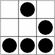
\includegraphics[width=0.25cm]{img/logo-glider.png}}

% % % en-tete et pieds de page configurables : fancyhdr.sty

% http://www.trustonme.net/didactels/250.html

% http://ww3.ac-poitiers.fr/math/tex/pratique/entete/entete.htm
% http://www.ctan.org/tex-archive/macros/latex/contrib/fancyhdr/fancyhdr.pdf
\usepackage{fancyhdr}
\pagestyle{fancy}
% \newcommand{\chaptermark}[1]{\markboth{#1}{}}
% \newcommand{\sectionmark}[1]{\markright{\thesection\ #1}}
\fancyhf{}
\fancyhead[LE,RO]{\bfseries\thepage}
\fancyhead[LO]{\bfseries\rightmark}
\fancyhead[RE]{\bfseries\leftmark}
\fancyfoot[LE]{\thepage /\pageref{LastPage} \hfill
	\scriptsize{\txtTITLE} % TITLE
\hfill \imgCORNER }
\fancyfoot[RO]{\imgCORNER \hfill
	\scriptsize{\txtTITLE} % TITLE
\hfill \thepage /\pageref{LastPage}}
\renewcommand{\headrulewidth}{0.5pt}
\renewcommand{\footrulewidth}{0.5pt}
\addtolength{\headheight}{0.5pt}
% \fancypagestyle{plain}{
	% \fancyhead{}
	% \renewcommand{\headrulewidth}{0pt}
% }

\usepackage{lettrine}
\usepackage{fancybox}

\title{\txtTITLE}
\date{ --- }

%============================= Corps =================================
\begin{document}

\setlength\parindent{0pt} % \noindent for all document

~\\

\vfill

\begin{center}
	\textbf{\Huge \txtTITLE}~\\~\\
	\textbf{\huge Ensure a job for life ;-)}~\\~\\
	\textbf{\large Roedy Green -- Canadian Mind Products~\footnote{\texttt{http://mindprod.com/jgloss/unmain.html} } }
\end{center}

\vfill

\tableofcontents

\clearpage

\section*{Introduction\markboth{Introduction}{Introduction}}
\addcontentsline{toc}{section}{Introduction}

\textit{Never ascribe to malice, that which can be explained by incompetence.} -- Napoleon~\\

In the interests of creating employment opportunities in the Java programming field, I am passing on these tips from the masters on how to write code that is so difficult to maintain, that the people who come after you will take years to make even the simplest changes. Further, if you follow all these rules religiously, you will even guarantee \textbf{yourself} a lifetime of employment, since no one but you has a hope in hell of maintaining the code. Then again, if you followed \textbf{all} these rules religiously, even you wouldn't be able to maintain the code!~\\ 

You don't want to overdo this. Your code should not \textbf{look} hopelessly unmaintainable, just \textbf{be} that way. Otherwise it stands the risk of being rewritten or refactored. 

\section*{General Principles\markboth{General Principles}{General Principles}}
\addcontentsline{toc}{section}{General Principles}

\textit{Quidquid latine dictum sit, altum sonatur. } -- Whatever is said in Latin sounds profound.~\\

To foil the maintenance programmer, you have to understand how he thinks. He has your giant program. He has no time to read it all, much less understand it. He wants to rapidly find the place to make his change, make it and get out and have no unexpected side effects from the change.~\\ 

He views your code through a toilet paper tube. He can only see a tiny piece of your program at a time. You want to make sure he can never get at the big picture from doing that. You want to make it as hard as possible for him to find the code he is looking for. But even more important, you want to make it as awkward as possible for him to safely \textbf{ignore} anything.~\\ 

Programmers are lulled into complacency by conventions. By every once in a while, by subtly violating convention, you force him to read every line of your code with a magnifying glass.~\\ 

You might get the idea that every language feature makes code unmaintainable -- not so, only if properly misused.

\section*{Naming\markboth{Naming}{Naming}}
\addcontentsline{toc}{section}{Naming}

\textit{"When I use a word," Humpty Dumpty said, in a rather scornful tone, "it means just what I choose it to mean -- neither more nor less."} -- Lewis Carroll --- Through the Looking Glass, Chapter 6~\\

Much of the skill in writing unmaintainable code is the art of naming variables and methods. They don't matter at all to the compiler. That gives you huge latitude to use them to befuddle the maintenance programmer.~\\~\\ 

\textbf{New Uses For \emph{Names For Baby}}~\\
Buy a copy of a baby naming book and you'll never be at a loss for variable names. Fred is a wonderful name, and easy to type. If you're looking for easy-to-type variable names, try \texttt{adsf} or \texttt{aoeu} if you type with a DSK keyboard.~\\ 

\textbf{Single Letter Variable Names}~\\
If you call your variables a, b, c, then it will be impossible to search for instances of them using a simple text editor. Further, nobody will be able to guess what they are for. If anyone even hints at breaking the tradition honoured since F\O RTRAN of using i, j, and k for indexing variables, namely replacing them with ii, jj and kk, warn them about what the Spanish Inquisition did to heretics.~\\ 

\clearpage

\textbf{Creative Miss-spelling}~\\
If you must use descriptive variable and function names, misspell them. By misspelling in some function and variable names, and spelling it correctly in others (such as SetPintleOpening SetPintalClosing) we effectively negate the use of grep or IDE search techniques. It works amazingly well. Add an international flavor by spelling \emph{tory} or \emph{tori} in different theatres/theaters.~\\ 

\textbf{Be Abstract}~\\
In naming functions and variables, make heavy use of abstract words like \emph{it}, \emph{everything}, \emph{data}, \emph{handle}, \emph{stuff}, \emph{do}, \emph{routine}, \emph{perform} and the digits e.g. \texttt{routineX48}, \texttt{PerformDataFunction}, \texttt{DoIt}, \texttt{HandleStuff} and \texttt{do\_args\_method}.~\\ 

\textbf{A.C.R.O.N.Y.M.S.}~\\
Use acronyms to keep the code terse. Real men never define acronyms; they understand them genetically.~\\ 

\textbf{Thesaurus Surrogatisation}~\\
To break the boredom, use a thesaurus to look up as much alternate vocabulary as possible to refer to the same action, e.g. \emph{display}, \emph{show}, \emph{present}. Vaguely hint there is some subtle difference, where none exists. However, if there are two similar functions that have a crucial difference, always use the same word in describing both functions (e.g. \emph{print} to mean "write to a file", "put ink on paper" and "display on the screen"). Under no circumstances, succumb to demands to write a glossary with the special purpose project vocabulary unambiguously defined. Doing so would be an unprofessional breach of the structured design principle of \emph{information hiding}.~\\ 

\textbf{Use Plural Forms From Other Languages}~\\
A VMS script kept track of the "statii" returned from various "Vaxen". Esperanto , Klingon~\footnote{\texttt{http://www.kli.org/}} and Hobbitese~\footnote{\texttt{http://www.chriswetherell.com/hobbit/}} qualify as languages for these purposes. For pseudo-Esperanto pluraloj, add oj. You will be doing your part toward world peace.~\\ 

\textbf{CapiTaliSaTion}~\\
Randomly capitalize the first letter of a syllable in the middle of a word. For example \texttt{ComputeRasterHistoGram()}.~\\ 

\textbf{Reuse Names}~\\
Wherever the rules of the language permit, give classes, constructors, methods, member variables, parameters and local variables the same names. For extra points, reuse local variable names inside \{\} blocks. The goal is to force the maintenance programmer to carefully examine the scope of every instance. In particular, in Java, make ordinary methods masquerade as constructors.~\\ 

\textbf{\AA ccented Letters}~\\
Use accented characters on variable names. E.g. \texttt{typedef struct \{ int i; \} {\'i}nt; } where the second {\'i}nt's {\'i} is actually i-acute. With only a simple text editor, it's nearly impossible to distinguish the slant of the accent mark.~\\ 

\textbf{Exploit Compiler Name Length Limits}~\\
If the compiler will only distinguish the first, say, 8 characters of names, then vary the endings e.g. \emph{var\_unit\_update()} in one case and \emph{var\_unit\_setup()} in another. The compiler will treat both as \emph{var\_unit}.~\\ 

\textbf{Underscore, a Friend Indeed}~\\
Use \_ and \_\_ as identifiers. ~\\

\textbf{Mix Languages}~\\
Randomly intersperse two languages (human or computer). If your boss insists you use his language, tell him you can organise your thoughts better in your own language, or, if that does not work, allege linguistic discrimination and threaten to sue your employers for a vast sum.~\\ 

\clearpage

\textbf{Extended ASCII}~\\
Extended ASCII characters are perfectly valid as variable names, including \ss , \DH , and {\~n} characters. They are almost impossible to type without copying/pasting in a simple text editor.~\\ 

\textbf{Names From Other Languages}~\\
Use foreign language dictionaries as a source for variable names. For example, use the German \emph{punkt} for \emph{point}. Maintenance coders, without your firm grasp of German, will enjoy the multicultural experience of deciphering the meaning.~\\ 

\textbf{Names From Mathematics}~\\
Choose variable names that masquerade as mathematical operators, e.g.: 
\begin{verbatim}
	openParen = (slash + asterix) / equals;
\end{verbatim}~\\

\textbf{Bedazzling Names}~\\
Choose variable names with irrelevant emotional connotation. e.g.: 
\begin{verbatim}
	marypoppins = (superman + starship) / god; 
\end{verbatim}
This confuses the reader because they have difficulty disassociating the emotional connotations of the words from the logic they're trying to think about.~\\ 

\textbf{Rename and Reuse}~\\
This trick works especially ell in Ada, a language immune to many of the standard obfuscation techniques. The people who originally named all the objects and packages you use were morons. Rather than try to convince them to change, just use renames and subtypes to rename everything to names of your own devising. Make sure to leave a few references to the old names in, as a trap for the unwary.~\\ 

\textbf{When To Use i}~\\
Never use i for the innermost loop variable. Use anything but. Use i liberally for any other purpose especially for non-int variables. Similarly use n as a loop index.~\\ 

\textbf{Conventions Schmentions}~\\
Ignore the Sun Java Coding Conventions~\footnote{\texttt{http://java.sun.com/docs/codeconv/}}, after all, Sun does. Fortunately, the compiler won't tattle when you violate them. The goal is to come up with names that differ subtlely only in case. If you are forced to use the capitalisation conventions, you can still subvert wherever the choice is ambigous, e.g. use \textbf{both} \emph{input\textbf{F}ile\textbf{n}ame} and \emph{input\textbf{f}ile\textbf{N}ame}. Invent your own hopelessly complex naming conventions, then berate everyone else for not following them.~\\ 

\textbf{Lower Case l Looks a Lot Like the Digit 1}~\\
Use lower case l to indicate long constants. e.g. 10l is more likely to be mistaken for 101 that 10L is. Ban any fonts that clearly disambiguate uvw wW gq9 2z 5s il17|!j oO08 `'" ;,. m nn rn {[()]}. Be creative.~\\ 

\textbf{Reuse of Global Names as Private}~\\
Declare a global array in module A, and a private one of the same name in the header file for module B, so that it appears that it's the global array you are using in module B, but it isn't. Make no reference in the comments to this duplication.~\\ 

\textbf{Recycling Revisited}~\\
Use scoping as confusingly as possible by recycling variable names in contradictory ways. For example, suppose you have global variables A and B, and functions foo and bar. If you know that variable A will be regularly passed to foo and B to bar, make sure to define the functions as function foo(B) and function bar(A) so that inside the functions A will always be referred to as B and vice versa. With more functions and globals, you can create vast confusing webs of mutually contradictory uses of the same names.~\\ 

\textbf{Recycle Your Variables}~\\
Wherever scope rules permit, reuse existing unrelated variable names. Similarly, use the same temporary variable for two unrelated purposes (purporting to save stack slots). For a fiendish variant, morph the variable, for example, assign a value to a variable at the top of a very long method, and then somewhere in the middle, change the meaning of the variable in a subtle way, such as converting it from a 0-based coordinate to a 1-based coordinate. Be certain not to document this change in meaning.~\\ 

\textbf{Cd wrttn wtht vwls s mch trsr}~\\
When using abbreviations inside variable or method names, break the boredom with several variants for the same word, and even spell it out longhand once in while. This helps defeat those lazy bums who use text search to understand only some aspect of your program. Consider variant spellings as a variant on the ploy, e.g. mixing International \emph{colour}, with American \emph{color} and dude-speak \emph{kulerz}. If you spell out names in full, there is only one possible way to spell each name. These are too easy for the maintenance programmer to remember. Because there are so many different ways to abbreviate a word, with abbreviations, you can have several different variables that all have the same apparent purpose. As an added bonus, the maintenance programmer might not even notice they are separate variables.~\\ 

\textbf{Misleading names}~\\
Make sure that every method does a little bit more (or less) than its name suggests. As a simple example, a method named \texttt{isValid(x)} should as a side effect convert x to binary and store the result in a database. ~\\

\textbf{m\_}~\\
A naming convention from the world of C++ is the use of "m\_" in front of members. This is supposed to help you tell them apart from methods, so long as you forget that "method" also starts with the letter "m".~\\ 

\textbf{o\_apple obj\_apple}~\\
Use an "o" or "obj" prefix for each instance of the class to show that you're thinking of the big, polymorphic picture.~\\ 

\textbf{Hungarian Notation}~\\
Hungarian Notation is the tactical nuclear weapon of source code obfuscation techniques; use it! Due to the sheer volume of source code contaminated by this idiom nothing can kill a maintenance engineer faster than a well planned Hungarian Notation attack. The following tips will help you corrupt the original intent of Hungarian Notation:~\\ 

\begin{minipage}[ht]{0.15\textwidth} ~\\ \end{minipage} \hfill \begin{minipage}[ht]{0.85\textwidth}
	Insist on using "c" for const in C++ and other languages that directly enforce the const-ness of a variable.~\\ 
	
	Seek out and use Hungarian warts that have meaning in languages other than your current language. For example insist on the PowerBuilder "l\_" and "a\_ " \{local and argument\} scoping prefixes and always use the VB-esque style of having a Hungarian wart for every control type when coding to C++. Try to stay ignorant of the fact that megs of plainly visible MFC source code does not use Hungarian warts for control types.~\\ 

	Always violate the Hungarian principle that the most commonly used variables should carry the least extra information around with them. Achieve this end through the techniques outlined above and by insisting that each class type have a custom wart prefix. Never allow anyone to remind you that \textbf{no} wart tells you that something \textbf{is} a class. The importance of this rule cannot be overstated if you fail to adhere to its principles the source code may become flooded with shorter variable names that have a higher vowel/consonant ratio. In the worst case scenario this can lead to a full collapse of obfuscation and the spontaneous reappearance of English Notation in code!~\\ 

	Flagrantly violate the Hungarian-esque concept that function parameters and other high visibility symbols must be given meaningful names, but that Hungarian type warts all by themselves make excellent temporary variable names.~\\ 
\end{minipage}~\\

\begin{minipage}[ht]{0.15\textwidth} ~\\ \end{minipage} \hfill \begin{minipage}[ht]{0.85\textwidth}
	Insist on carrying outright orthogonal information in your Hungarian warts. Consider this real world example "a\_crszkvc30LastNameCol". It took a team of maintenance engineers nearly 3 days to figure out that this whopper variable name described a const, reference, function argument that was holding information from a database column of type Varchar[30] named "LastName" which was part of the table's primary key. When properly combined with the principle that "all variables should be public" this technique has the power to render thousands of lines of source code obsolete instantly!~\\ 
	
	Use to your advantage the principle that the human brain can only hold 7 pieces of information concurrently. For example code written to the above standard has the following properties: 
	\begin{itemize}
		\item a single assignment statement carries 14 pieces of type and name information. 
		\item a single function call that passes three parameters and assigns a result carries 29 pieces of type and name information. 
		\item Seek to improve this excellent, but far too concise, standard. Impress management and coworkers by recommending a 5 letter day of the week prefix to help isolate code written on 'Monam' and 'FriPM'. 
		\item It is easy to overwhelm the short term memory with even a moderately complex nesting structure, \textbf{especially} when the maintenance programmer can't see the start and end of each block on screen simultaneously. 
	\end{itemize}
\end{minipage}~\\~\\

\textbf{Hungarian Notation Revisited}~\\
One followon trick in the Hungarian notation is "change the type of a variable but leave the variable name unchanged". This is almost invariably done in windows apps with the migration from Win16 :- WndProc(HWND hW, WORD wMsg, WORD wParam, LONG lParam) to Win32 WndProc(HWND hW, UINT wMsg, WPARAM wParam, LPARAM lParam) where the w values hint that they are words, but they really refer to longs. The real value of this approach comes clear with the Win64 migration, when the parameters will be 64 bits wide, but the old "w" and "l" prefixes will remain forever.~\\ 

\textbf{Reduce, Reuse, Recycle}~\\
If you have to define a structure to hold data for callbacks, always call the structure PRIVDATA. Every module can define it's own PRIVDATA. In VC++, this has the advantage of confusing the debugger so that if you have a PRIVDATA variable and try to expand it in the watch window, it doesn't know which PRIVDATA you mean, so it just picks one.~\\ 

\textbf{Obscure film references}~\\
Use constant names like \texttt{LancelotsFavouriteColour} instead of \textbf{blue} and assign it hex value of \$0204FB. The color looks identical to pure blue on the screen, and a maintenance programmer would have to work out 0204FB (or use some graphic tool) to know what it looks like. Only someone intimately familiar with Monty Python and the Holy Grail would know that Lancelot's favorite color was blue. If a maintenance programmer can't quote entire Monty Python movies from memory, he or she has no business being a programmer.

\section*{Camouflage\markboth{Camouflage}{Camouflage}}
\addcontentsline{toc}{section}{Camouflage}

\textit{The longer it takes for a bug to surface, the harder it is to find. } -- Roedy Green

Much of the skill in writing unmaintainable code is the art of camouflage, hiding things, or making things appear to be what they are not. Many depend on the fact the compiler is more capable at making fine distinctions than either the human eye or the text editor. Here are some of the best camouflaging techniques.~\\
 
\textbf{Code That Masquerades As Comments and Vice Versa}~\\
Include sections of code that is commented out but at first glance does not appear to be. 
	\begin{verbatim}
		for(j=0; j<array_len; j+ =8) 
			{ 
			total += array[j+0 ]; 
			total += array[j+1 ]; 
			total += array[j+2 ];/* Main body of 
			total += array[j+3]; * loop is unrolled 
			total += array[j+4]; * for greater speed. 
			total += array[j+5]; */ 
			total += array[j+6 ]; 
			total += array[j+7 ]; 
			} 
	\end{verbatim}
Without the colour coding would you notice that three lines of code are commented out?~\\ 

\textbf{namespaces}~\\
Struct/union and typedef struct/union are different name spaces in C (not in C++). Use the same name in both name spaces for structures or unions. Make them, if possible, nearly compatible. 
	\begin{verbatim}
		typedef struct { 
		char* pTr; 
		size_t lEn; 
		} snafu; 
		struct snafu { 
		unsigned cNt 
		char* pTr; 
		size_t lEn; 
		} A; 
	\end{verbatim}

\textbf{Hide Macro Definitions}~\\
Hide macro definitions in amongst rubbish comments. The programmer will get bored and not finish reading the comments thus never discover the macro. Ensure that the macro replaces what looks like a perfectly legitimate assignment with some bizarre operation, a simple example: 
	\begin{verbatim}
		#define a=b a=0-b 
	\end{verbatim}

\textbf{Look Busy}~\\
use define statements to make made up functions that simply comment out their arguments, e.g.: 
\begin{verbatim}
	#define fastcopy(x,y,z) /*xyz*/ 
	... 
	fastcopy(array1, array2, size); /* does nothing */ 
\end{verbatim}

\textbf{Use Continuation to hide variables}~\\
Instead of using \texttt{\#define local\_var xy\_z} break up "xy\_z" onto two lines: 
\begin{verbatim}
	#define local_var xy\ 
	_z // local_var OK 
\end{verbatim}
That way a global search for xy\_z will come up with nothing for that file. To the C preprocessor, the "\" at the end of the line means glue this line to the next one.~\\ 

\textbf{Arbitrary Names That Masquerade as Keywords}~\\
When documenting, and you need an arbitrary name to represent a filename use "\emph{file}". Never use an obviously arbitrary name like "\emph{Charlie.dat}" or "\emph{Frodo.txt}". In general, in your examples, use arbitrary names that sound as much like reserved keywords as possible. For example, good names for parameters or variables would be "\emph{bank}", "\emph{blank}", "\emph{class}", "\emph{const}", "\emph{constant}", "\emph{input}", "\emph{key}", "\emph{keyword}", "\emph{kind}", "\emph{output}", "\emph{parameter}" "\emph{parm}", "\emph{system}", "\emph{type}", "\emph{value}", "\emph{var}" and "\emph{variable}". If you use actual reserved words for your arbitrary names, which would be rejected by your command processor or compiler, so much the better. If you do this well, the users will be hopelessly confused between reserved keywords and arbitrary names in your example, but you can look innocent, claiming you did it to help them associate the appropriate purpose with each variable.~\\ 

\clearpage

\textbf{Code Names Must Not Match Screen Names}~\\
Choose your variable names to have absolutely no relation to the labels used when such variables are displayed on the screen. E.g. on the screen label the field "\emph{Postal Code}" but in the code call the associated variable "\emph{zip}".~\\ 

\textbf{Don't Change Names}~\\
Instead of globally renaming to bring two sections of code into sync, use multiple TYPEDEFs of the same symbol. ~\\

\textbf{How to Hide Forbidden Globals}~\\
Since global variables are "evil", define a structure to hold all the things you'd put in globals. Call it something clever like EverythingYoullEverNeed. Make all functions take a pointer to this structure (call it handle to confuse things more). This gives the impression that you're not using global variables, you're accessing everything through a "handle". Then declare one statically so that all the code is using the same copy anyway. ~\\

\textbf{Hide Instances With Synonyms}~\\
Maintenance programmers, in order to see if they'll be any cascading effects to a change they make, do a global search for the variables named. This can be defeated by this simple expedient of having synonyms, such as 
\begin{verbatim}
	#define xxx global_var // in file std.h 
	#define xy_z xxx // in file ..\O ther\substd.h 
	#define local_var xy_z // in file ..\codestd\inst.h
\end{verbatim} 
These defs should be scattered through different include-files. They are especially effective if the include-files are located in different directories. The other technique is to reuse a name in every scope. The compiler can tell them apart, but a simple minded text searcher cannot. Unfortunately SCIDs in the coming decade will make this simple technique impossible. since the editor understands the scope rules just as well as the compiler.~\\ 

\textbf{Long Similar Variable Names}~\\
Use very long variable names or class names that differ from each other by only one character, or only in upper/lower case. An ideal variable name pair is \texttt{swimmer} and \texttt{swimner}. Exploit the failure of most fonts to clearly discriminate between \texttt{ilI1|} or \texttt{oO08} with identifier pairs like \texttt{parselnt} and \texttt{parseInt} or \texttt{D0Calc} and \texttt{DOCalc}. l is an exceptionally fine choice for a variable name since it will, to the casual glance, masquerade as the constant 1. In many fonts rn looks like an m. So how about a variable swirnrner. Create variable names that differ from each other only in case e.g. HashTable and Hashtable.~\\ 

\textbf{Similar-Sounding Similar-Looking Variable Names}~\\
Although we have one variable named xy\_z, there's certainly no reason not to have many other variables with similar names, such as xy\_Z, xy\_\_z, \_xy\_z, \_xyz, XY\_Z, xY\_z, and Xy\_z.~\\ 
Variables that resemble others except for capitalization and underlines have the advantage of confounding those who like remembering names by sound or letter-spelling, rather than by exact representations.~\\ 

\textbf{Overload and Bewilder}~\\
In C++, overload library functions by using \#define. That way it looks like you are using a familiar library function where in actuality you are using something totally different.~\\ 

\textbf{Choosing The Best Overload Operator}~\\
In C++, overload +,-,*,/ to do things totally unrelated to addition, subtraction etc. After all, if the Stroustroup can use the shift operator to do I/O, why should you not be equally creative? If you overload +, make sure you do it in a way that $i = i + 5$; has a totally different meaning from $i += 5$; Here is an example of elevating overloading operator obfuscation to a high art. Overload the '!' operator for a class, but have the overload have nothing to do with inverting or negating. Make it return an integer. Then, in order to get a logical value for it, you must use '! !'. However, this inverts the logic, so [drum roll] you must use '! ! !'. Don't confuse the ! operator, which returns a boolean 0 or 1, with the \~{} bitwise logical negation operator.~\\ 

\clearpage

\textbf{Overload new}~\\
Overload the "new" operator -- much more dangerous than overloading the +-/*. This can cause total havoc if overloaded to do something different from it's original function (but vital to the object's function so it's very difficult to change). This should ensure users trying to create a dynamic instance get really stumped. You can combine this with the case sensitivity trickalso have a member function, and variable called "New".~\\ 
\begin{verbatim}
	#define
	#define in C++ deserves an entire essay on its own to explore its rich possibilities for obfuscation. Use lower case #define variables so they masquerade as ordinary variables. Never use parameters to your preprocessor functions. Do everything with global #defines. One of the most imaginative uses of the preprocessor I have heard of was requiring five passes through CPP before the code was ready to compile. Through clever use of defines and ifdefs, a master of obfuscation can make header files declare different things depending on how many times they are included. This becomes especially interesting when one header is included in another header. Here is a particularly devious example: 
	#ifndef DONE 
	
	#ifdef TWICE 
	
	// put stuff here to declare 3rd time around 
	void g(char* str); 
	#define DONE 
	
	#else // TWICE 
	#ifdef ONCE 
	
	// put stuff here to declare 2nd time around 
	void g(void* str); 
	#define TWICE 
	
	#else // ONCE 
	
	// put stuff here to declare 1st time around 
	void g(std::string str); 
	#define ONCE 
	
	#endif // ONCE 
	#endif // TWICE 
	#endif // DONE
\end{verbatim}
This one gets fun when passing g() a char*, because a different version of g() will be called depending on how many times the header was included.~\\ 

\textbf{Compiler Directives}~\\
Compiler directives were designed with the express purpose of making the same code behave completely differently. Turn the boolean short-circuiting directive on and off repeatedly and vigourously, as well as the long strings directive.~\\ 

\clearpage

\section*{Documentation\markboth{Documentation}{Documentation}}
\addcontentsline{toc}{section}{Documentation}

\textit{Any fool can tell the truth, but it requires a man of some sense to know how to lie well.} -- Samuel Butler (1835 - 1902)~\\

\textit{Incorrect documentation is often worse than no documentation. } -- Bertrand Meyer~\\

Since the computer ignores comments and documentation, you can lie outrageously and do everything in your power to befuddle the poor maintenance programmer.~\\ 

\textbf{Lie in the comments}~\\
You don't have to actively lie, just fail to keep comments as up to date with the code.~\\ 

\textbf{Document the obvious}~\\
Pepper the code with comments like \texttt{/* add 1 to i */} however, never document wooly stuff like the overall purpose of the package or method.~\\ 

\textbf{Document How Not Why}~\\
Document only the details of what a program does, not what it is attempting to accomplish. That way, if there is a bug, the fixer will have no clue what the code should be doing.~\\ 

\textbf{Avoid Documenting the "Obvious"}~\\
If, for example, you were writing an airline reservation system, make sure there are at least 25 places in the code that need to be modified if you were to add another airline. Never document where they are. People who come after you have no business modifying your code without thoroughly understanding every line of it.~\\ 

\textbf{On the Proper Use Of Documentation Templates}~\\
Consider function documentation prototypes used to allow automated documentation of the code. These prototypes should be copied from one function (or method or class) to another, but never fill in the fields. If for some reason you are forced to fill in the fields make sure that all parameters are named the same for all functions, and all cautions are the same but of course not related to the current function at all.~\\ 

\textbf{On the Proper Use of Design Documents}~\\
When implementing a very complicated algorithm, use the classic software engineering principles of doing a sound design before beginning coding. Write an extremely detailed design document that describes each step in a very complicated algorithm. The more detailed this document is, the better.~\\
 
In fact, the design doc should break the algorithm down into a hierarchy of structured steps, described in a hierarchy of auto-numbered individual paragraphs in the document. Use headings at least 5 deep. Make sure that when you are done, you have broken the structure down so completely that there are over 500 such auto-numbered paragraphs. For example, one paragraph might be(this is a real example)~\\ 

1.2.4.6.3.13 - Display all impacts for activity where selected mitigations can apply (short pseudocode omitted).~\\ 

then... (and this is the kicker) when you write the code, for each of these paragraphs you write a corresponding global function named:~\\ 
\begin{verbatim}
	Act1_2_4_6_3_13()
\end{verbatim} 
Do not document these functions. After all, that's what the design document is for!~\\
 
Since the design doc is auto-numbered, it will be extremely difficult to keep it up to date with changes in the code (because the function names, of course, are static, not auto-numbered.) This isn't a problem for you because you will not try to keep the document up to date. In fact, do everything you can to destroy all traces of the document.~\\ 

Those who come after you should only be able to find one or two contradictory, early drafts of the design document hidden on some dusty shelving in the back room near the dead 286 computers.~\\ 

\textbf{Units of Measure}~\\
Never document the units of measure of any variable, input, output or parameter. e.g. feet, metres, cartons. This is not so important in bean counting, but it is very important in engineering work. As a corollary, never document the units of measure of any conversion constants, or how the values were derived. It is mild cheating, but very effective, to salt the code with some incorrect units of measure in the comments. If you are feeling particularly malicious, make up your own unit of measure; name it after yourself or some obscure person and never define it. If somebody challenges you, tell them you did so that you could use integer rather than floating point arithmetic.~\\ 

\textbf{Gotchas}~\\
Never document gotchas in the code. If you suspect there may be a bug in a class, keep it to yourself. If you have ideas about how the code should be reorganised or rewritten, for heaven's sake, do not write them down. Remember the words of Thumper in the movie Bambi "\emph{If you can't say anything nice, don't say anything at all}". What if the programmer who wrote that code saw your comments? What if the owner of the company saw them? What if a customer did? You could get yourself fired. An anonymous comment that says "This needs to be fixed!" can do wonders, especially if it's not clear what the comment refers to. Keep it vague, and nobody will feel personally criticised.~\\ 

\textbf{Documenting Variables}~\\
Never put a comment on a variable declaration. Facts about how the variable is used, its bounds, its legal values, its implied/displayed number of decimal points, its units of measure, its display format, its data entry rules (e.g. total fill, must enter), when its value can be trusted etc. should be gleaned from the procedural code. If your boss forces you to write comments, lard method bodies with them, but never comment a variable declaration, not even a temporary!~\\ 

\textbf{Disparage In the Comments}~\\
Discourage any attempt to use external maintenance contractors by peppering your code with insulting references to other leading software companies, especial anyone who might be contracted to do the work. e.g.:
\begin{verbatim}
	/* The optimised inner loop. 
	This stuff is too clever for the dullard at Software Services Inc., who would 
	probably use 50 times as memory & time using the dumb routines in <math.h>. 
	*/ 
	class clever_SSInc 
	{ 
	... 
	}
\end{verbatim}
If possible, put insulting stuff in syntactically significant parts of the code, as well as just the comments so that management will probably break the code if they try to sanitise it before sending it out for maintenance. ~\\

\textbf{COMMENT AS IF IT WERE C\O B\O L ON PUNCH CARDS}~\\
Always refuse to accept advances in the development environment arena, especially SCIDs. Disbelieve rumors that all function and variable declarations are never more than one click away and always assume that code developed in Visual Studio 6.0 will be maintained by someone using edlin or vi. Insist on Draconian commenting rules to bury the source code proper.~\\ 

\textbf{Monty Python Comments}~\\
On a method called makeSnafucated insert only the JavaDoc \emph{/* make snafucated */}. Never define what snafucated means anywhere. Only a fool does not already know, with complete certainty, what snafucated means. For classic examples of this technique, consult the Sun AWT JavaDOC.~\\ 

\section*{Program Design\markboth{Program Design}{Program Design}}
\addcontentsline{toc}{section}{Program Design}

\textit{The cardinal rule of writing unmaintainable code is to specify each fact in as many places as possible and in as many ways as possible.} -- Roedy Green~\\

The key to writing maintainable code is to specify each fact about the application in only one place. To change your mind, you need change it in only one place, and you are guaranteed the entire program will still work. Therefore, the key to writing unmaintainable code is to specify a fact over and over, in as many places as possible, in as many variant ways as possible. Happily, languages like Java go out of their way to make writing this sort of unmaintainable code easy. For example, it is almost impossible to change the type of a widely used variable because all the casts and conversion functions will no longer work, and the types of the associated temporary variables will no longer be appropriate. Further, if the variable is displayed on the screen, all the associated display and data entry code has to be tracked down and manually modified. The Algol family of languages which include C and Java treat storing data in an array, Hashtable, flat file and database with \textbf{totally} different syntax. In languages like Abundance, and to some extent Smalltalk, the syntax is identical; just the declaration changes. Take advantage of Java's ineptitude. Put data you know will grow too large for RAM, for now into an array. That way the maintenance programmer will have a horrendous task converting from array to file access later. Similarly place tiny files in databases so the maintenance programmer can have the fun of converting them to array access when it comes time to performance tune.~\\ 

\textbf{Java Casts}~\\
Java's casting scheme is a gift from the Gods. You can use it without guilt since the language requires it. Every time you retrieve an object from a Collection you must cast it back to its original type. Thus the type of the variable may be specified in dozens of places. If the type later changes, all the casts must be changed to match. The compiler may or may not detect if the hapless maintenance programmer fails to catch them all (or changes one too many). In a similar way, all matching casts to \texttt{(short)} need to be changed to \texttt{(int)} if the type of a variable changes from \texttt{short} to \texttt{int}. There is a movement afoot in invent a generic cast operator \texttt{(cast)} and a generic conversion operator \texttt{(convert)} that would require no maintenance when the type of variable changes. Make sure this heresy never makes it into the language specification. Vote no on RFE 114691 and on genericity which would eliminate the need for many casts. ~\\

\textbf{Exploit Java's Redundancy}~\\
Java insists you specify the type of every variable twice. Java programmers are so used to this redundancy they won't notice if you make the two types slightly different, as in this example: \texttt{Bubblegum b = new Bubblegom();}~\\

Unfortunately the popularity of the ++ operator makes it harder to get away with pseudo-redundant code like this: \texttt{swimmer = swimner + 1;}~\\ 

\textbf{Never Validate}~\\
Never check input data for any kind of correctness or discrepancies. It will demonstrate that you absolutely trust the company's equipment as well as that you are a perfect team player who trusts all project partners and system operators. Always return reasonable values even when data inputs are questionable or erroneous.~\\ 

\textbf{Be polite, Never Assert}~\\
Avoid the assert() mechanism, because it could turn a three-day debug fest into a ten minute one.~\\ 

\textbf{Avoid Encapsulation}~\\
In the interests of efficiency, avoid encapsulation. Callers of a method need all the external clues they can get to remind them how the method works inside.~\\ 

\textbf{Clone \& Modify}~\\
In the name of efficiency, use cut/paste/clone/modify. This works much faster than using many small reusable modules. This is especially useful in shops that measure your progress by the number of lines of code you've written.~\\ 

\clearpage

\textbf{Use Static Arrays}~\\
If a module in a library needs an array to hold an image, just define a static array. Nobody will ever have an image bigger than 512 x 512, so a fixed-size array is OK. For best precision, make it an array of doubles. Bonus effect for hiding a 2 Meg static array which causes the program to exceed the memory of the client's machine and thrash like crazy even if they never use your routine.~\\ 

\textbf{Dummy Interfaces}~\\
Write an empty interface called something like "WrittenByMe", and make all of your classes implement it. Then, write wrapper classes for any of Java's built-in classes that you use. The idea is to make sure that every single object in your program implements this interface. Finally, write all methods so that both their arguments and return types are WrittenByMe. This makes it nearly impossible to figure out what some methods do, and introduces all sorts of entertaining casting requirements. For a further extension, have each team member have his/her own personal interface (e.g., WrittenByJoe); any class worked on by a programmer gets to implement his/her interface. You can then arbitrary refer to objects by any one of a large number of meaningless interfaces!~\\ 

\textbf{Giant Listeners}~\\
Never create separate Listeners for each Component. Always have one listener for every button in your project and simply use massive if...else statements to test for which button was pressed.~\\ 

\textbf{Too Much Of A Good Thing~\texttrademark}~\\
Go wild with encapsulation and oo. For example, That one probably did not even seem funny.~\\Don't worry. It will some day.
\begin{verbatim}
	myPanel.add( getMyButton() ); 
	private JButton getMyButton() 
		{ return myButton; } 
\end{verbatim}

\textbf{Friendly Friend}~\\
Use as often as possible the friend-declaration in C++. Combine this with handing the pointer of the creating class to a created class. Now you don't need to fritter away your time in thinking about interfaces. Additionally you should use the keywords private and protected to prove that your classes are well encapsulated.~\\ 

\textbf{Use Three Dimensional Arrays}~\\
Lots of them. Move data between the arras in convoluted ways, say, filling the columns in arrayB with the rows from arrayA. Doing it with an offset of 1, for no apparent reason, is a nice touch. Makes the maintenance programmer nervous.~\\ 

\textbf{Mix and Match}~\\
Use both accessor methods and public variables. That way, you can change an object's variable without the overhead of calling the accessor, but still claim that the class is a "Java Bean". This has the additional advantage of frustrating the maintenence programmer who adds a logging function to try to figure out who is changing the value.~\\ 

\textbf{Wrap, wrap, wrap}~\\
Whenever you have to use methods in code you did not write, insulate your code from that other dirty code by at least one layer of wrapper. After all, the other author \textbf{might} some time in the future recklessly rename every method. Then where would you be? You could of course, if he did such a thing, insulate your code from the changes by writing a wrapper or you could let VAJ handle the global rename. However, this is the perfect excuse to preemptively cut him off at the pass with a wrapper layer of indirection, \textbf{before} he does anything idiotic. One of Java's main faults is that there is no way to solve many simple problems without dummy wrapper methods that do nothing but call another method of the same name, or a closely related name. This means it is possible to write wrappers four-levels deep that do absolutely nothing, and almost no one will notice. To maximise the obscuration, at each level, rename the methods, selecting random synonyms from a thesaurus. This gives the illusion something of note is happening. Further, the renaming helps ensure the lack of consistent project terminology. To ensure no one attempts to prune your levels back to a reasonable number, invoke some of your code bypassing the wrappers at each of the levels.~\\ 

\textbf{Wrap Wrap Wrap Some More}~\\
Make sure all API functions are wrapped at least 6-8 times, with function definitions in separate source files. Using \texttt{\#defines} to make handy shortcuts to these functions also helps.~\\ 

\textbf{No Secrets!}~\\
Declare every method and variable public. After all, somebody, sometime might want to use it. Once a method has been declared public, it can't very well be retracted, now can it? This makes it very difficult to later change the way anything works under the covers. It also has the delightful side effect of obscuring what a class is for. If the boss asks if you are out of your mind, tell him you are following the classic principles of transparent interfaces.~\\ 

\textbf{The Kama Sutra}~\\
This technique has the added advantage of driving any users or documenters of the package to distraction as well as the maintenance programmers. Create a dozen overloaded variants of the same method that differ in only the most minute detail. I think it was Oscar Wilde who observed that positions 47 and 115 of the Kama Sutra were the same except in 115 the woman had her fingers crossed. Users of the package then have to carefully peruse the long list of methods to figure out just which variant to use. The technique also balloons the documentation and thus ensures it will more likely be out of date. If the boss asks why you are doing this, explain it is solely for the convenience of the users. Again for the full effect, clone any common logic and sit back and wait for it the copies to gradually get out of sync.~\\ 

\textbf{Permute and Baffle}~\\
Reverse the parameters on a method called drawRectangle(height, width) to drawRectangle(width, height) without making any change whatsoever to the name of the method. Then a few releases later, reverse it back again. The maintenance programmers can't tell by quickly looking at any call if it has been adjusted yet. Generalisations are left as an exercise for the reader.~\\ 

\textbf{Theme and Variations}~\\
Instead of using a parameter to a single method, create as many separate methods as you can. For example instead of setAlignment(int alignment) where alignment is an enumerated constant, for left, right, center, create three methods setLeftAlignment, setRightAlignment, and setCenterAlignment. Of course, for the full effect, you must clone the common logic to make it hard to keep in sync.~\\ 

\textbf{Static Is Good}~\\
Make as many of your variables as possible static. If you don't need more than one instance of the class in this program, no one else ever will either. Again, if other coders in the project complain, tell them about the execution speed improvement you're getting.~\\ 

\textbf{Cargill's Quandry}~\\
Take advantage of Cargill's quandary (I think this was his) "any design problem can be solved by adding an additional level of indirection, except for too many levels of indirection." Decompose OO programs until it becomes nearly impossible to find a method which actually updates program state. Better yet, arrange all such occurrences to be activated as callbacks from by traversing pointer forests which are known to contain every function pointer used within the entire system. Arrange for the forest traversals to be activated as side-effects from releasing reference counted objects previously created via deep copies which aren't really all that deep.~\\ 

\textbf{Packratting}~\\
Keep all of your unused and outdated methods and variables around in your code. After all - if you needed to use it once in 1976, who knows if you will want to use it again sometime? Sure the program's changed since then, but it might just as easily change back, you "don't want to have to reinvent the wheel" (supervisors love talk like that). If you have left the comments on those methods and variables untouched, and sufficiently cryptic, anyone maintaining the code will be too scared to touch them.~\\ 

\clearpage

\textbf{And That's Final}~\\
Make all of your leaf classes final. After all, you're done with the project - certainly no one else could possibly improve on your work by extending your classes. And it might even be a security flaw - after all, isn't java.lang.String final for just this reason? If other coders in your project complain, tell them about the execution speed improvement you're getting.~\\ 

\textbf{Eschew The Interface}~\\
In Java, disdain the interface. If your supervisors complain, tell them that Java interfaces force you to "cut-and-paste" code between different classes that implement the same interface the same way, and they know how hard that would be to maintain. Instead, do as the Java AWT designers did - put lots of functionality in your classes that can only be used by classes that inherit from them, and use lots of "instanceof" checks in your methods. This way, if someone wants to reuse your code, they have to extend your classes. If they want to reuse your code from two different classes - tough luck, they can't extend both of them at once! If an interface is unavoidable, make an all-purpose one and name it something like "ImplementableIface." Another gem from academia is to append "Impl" to the names of classes that implement interfaces. This can be used to great advantage, e.g. with classes that implement Runnable.~\\ 

\textbf{Avoid Layouts}~\\
Never use layouts. That way when the maintenance programmer adds one more field he will have to manually adjust the absolute co-ordinates of every other thing displayed on the screen. If your boss forces you to use a layout, use a single giant GridBagLayout, and hard code in absolute grid co-ordinates.~\\ 

\textbf{Environment variables}~\\
If you have to write classes for some other programmer to use, put environment-checking code (getenv() in C++ / System.getProperty() in Java) in your classes' nameless static initializers, and pass all your arguments to the classes this way, rather than in the constructor methods. The advantage is that the initializer methods get called as soon as the class program binaries get loaded, even before any of the classes get instantiated, so they will usually get executed before the program main(). In other words, there will be no way for the rest of the program to modify these parameters before they get read into your classes - the users better have set up all their environment variables just the way you had them!~\\ 

\textbf{Table Driven Logic}~\\
Eschew any form of table-driven logic. It starts out innocently enough, but soon leads to end users proofreading and then shudder, even modifying the tables for themselves.~\\ 

\textbf{Modify Mom's Fields}~\\
In Java, all primitives passed as parameters are effectively read-only because they are passed by value. The callee can modify the parameters, but that has no effect on the caller's variables. In contrast all objects passed are read-write. The reference is passed by value, which means the object itself is effectively passed by reference. The callee can do whatever it wants to the fields in your object. Never document whether a method actually modifies the fields in each of the passed parameters. Name your methods to suggest they only look at the fields when they actually change them.~\\ 

\textbf{The Magic Of Global Variables}~\\
Instead of using exceptions to handle error processing, have your error message routine set a global variable. Then make sure that every long-running loop in the system checks this global flag and terminates if an error occurs. Add another global variable to signal when a user presses the 'reset' button. Of course all the major loops in the system also have to check this second flag. Hide a few loops that don't terminate on demand.~\\ 

\textbf{Globals, We Can't Stress These Enough!}~\\
If God didn't want us to use global variables, he wouldn't have invented them. Rather than disappoint God, use and set as many global variables as possible. Each function should use and set at least two of them, even if there's no reason to do this. After all, any good maintenance programmer will soon figure out this is an exercise in detective work, and she'll be happy for the exercise that separates real maintenance programmers from the dabblers.~\\ 

\textbf{Globals, One More Time, Boys}~\\
Global variables save you from having to specify arguments in functions. Take full advantage of this. Elect one or more of these global variables to specify what kinds of processes to do on the others. Maintenance programmers foolishly assume that C functions will not have side effects. Make sure they squirrel results and internal state information away in global variables.~\\ 

\textbf{Side Effects}~\\
In C, functions are supposed to be idempotent, (without side effects). I hope that hint is sufficient. ~\\

\textbf{Backing Out}~\\
Within the body of a loop, assume that the loop action is successful and immediately update all pointer variables. If an exception is later detected on that loop action, back out the pointer advancements as side effects of a conditional expression following the loop body.~\\ 

\textbf{Local Variables}~\\
Never use local variables. Whenever you feel the temptation to use one, make it into an instance or static variable instead to unselfishly share it with all the other methods of the class. This will save you work later when other methods need similar declarations. C++ programmers can go a step further by making all variables global.~\\ 

\textbf{Reduce, Reuse, Recycle}~\\
If you have to define a structure to hold data for callbacks, always call the structure PRIVDATA. Every module can define it's own PRIVDATA. In VC++, this has the advantage of confusing the debugger so that if you have a PRIVDATA variable and try to expand it in the watch window, it doesn't know which PRIVDATA you mean, so it just picks one.~\\ 

\textbf{Configuration Files}~\\
These usually have the form keyword=value. The values are loaded into Java variables at load time. The most obvious obfuscation technique is to use slightly different names for the keywords and the Java variables. Use configuration files even for constants that never change at run time. Parameter file variables require at least five times as much code to maintain as a simple variable would. ~\\

\textbf{Bloated classes}~\\
To ensure your classes are bounded in the most obtuse way possible, make sure you include peripheral, obscure methods and attributes in every class. For example, a class that defines astrophysical orbit geometry really should have a method that computes ocean tide schedules and attributes that comprise a Crane weather model. Not only does this over-define the class, it makes finding these methods in the general system code like looking for a guitar pick in a landfill. ~\\

\textbf{Subclass With Abandon}~\\
Object oriented programming is a godsend for writing unmaintainable code. If you have a class with 10 properties (member/method) in it, consider a base class with only one property and subclassing it 9 levels deep so that each descendant adds one property. By the time you get to the last descendant class, you'll have all 10 properties. If possible, put each class declaration in a separate file. This has the added effect of bloating your INCLUDE or USES statements, and forces the maintainer to open that many more files in his or her editor. Make sure you create at least one instance of each subclass. ~\\

\clearpage

\section*{Coding Obfuscation\markboth{Coding Obfuscation}{Coding Obfuscation}}
\addcontentsline{toc}{section}{Coding Obfuscation}

\textit{Sedulously eschew obfuscatory hyperverbosity and prolixity.}~\\
 
\textbf{Obfuscated C}~\\
Follow the obfuscated C contests on the Internet and sit at the lotus feet of the masters. ~\\

\textbf{Find a Forth or APL Guru}~\\
In those worlds, the terser your code and the more bizarre the way it works, the more you are revered. ~\\

\textbf{I'll Take a Dozen}~\\
Never use one housekeeping variable when you could just as easily use two or three. ~\\

\textbf{Jude the Obscure}~\\
Always look for the most obscure way to do common tasks. For example, instead of using arrays to convert an integer to the corresponding string, use code like this: 
\begin{verbatim}
	char *p; 
	switch (n) 
	{ 
	case 1: 
	    p = "one"; 
	    if (0) 
	case 2: 
	    p = "two"; 
	    if (0) 
	case 3: 
	    p = "three"; 
	    printf("\%s", p); 
	    break; 
	}
\end{verbatim}

\textbf{Foolish Consistency Is the Hobgoblin of Little Minds}~\\
When you need a character constant, use many different formats ' ', 32, 0x20, 040. Make liberal use of the fact that 10 and 010 are not the same number in C or Java.~\\ 

\textbf{Casting}~\\
Pass all data as a void * and then typecast to the appropriate structure. Using byte offsets into the data instead of structure casting is fun too. ~\\

\textbf{The Nested Switch}~\\
(a switch within a switch) is the most difficult type of nesting for the human mind to unravel. ~\\

\textbf{Exploit Implicit Conversion}~\\
Memorize all of the subtle implicit conversion rules in the programming language. Take full advantage of them. Never use a picture variable (in COBOL or PL/I) or a general conversion routine (such as sprintf in C). Be sure to use floating-point variables as indexes into arrays, characters as loop counters, and perform string functions on numbers. After all, all of these operations are well-defined and will only add to the terseness of your source code. Any maintainer who tries to understand them will be very grateful to you because they will have to read and learn the entire chapter on implicit data type conversion; a chapter that they probably had completely overlooked before working on your programs. ~\\

\textbf{Raw ints}~\\
When using ComboBoxes, use a switch statement with integer cases rather than named constants for the possible values. ~\\

\textbf{Semicolons!}~\\
Always use semicolons whenever they are syntactically allowed. For example: 
\begin{verbatim}
	if(a); 
	else; 
	{ 
	int d; 
	d = c; 
	} 
	; 
\end{verbatim}

\textbf{Use Octal}~\\
Smuggle octal literals into a list of decimal numbers like this: 
\begin{verbatim}
	array = new int [] 
	{ 
	111, 
	120, 
	013, 
	121, 
	};
\end{verbatim}

\textbf{Convert Indirectly}~\\
Java offers great opportunity for obfuscation whenever you have to convert. As a simple example, if you have to convert a double to a String, go circuitously, via Double with \texttt{new Double(d).toString()} rather than the more direct \texttt{Double.toString(d)}. You can, of course, be far more circuitous than that! Avoid any conversion techniques recommended by the Conversion Amanuensis. You get bonus points for every extra temporary object you leave littering the heap after your conversion.~\\ 

\textbf{Nesting}~\\
Nest as deeply as you can. Good coders can get up to 10 levels of ( ) on a single line and 20 { } in a single method. C++ coders have the additional powerful option of preprocessor nesting totally independent of the nest structure of the underlying code. You earn extra Brownie points whenever the beginning and end of a block appear on separate pages in a printed listing. Wherever possible, convert nested ifs into nested [? ] ternaries. If they span several lines, so much the better.~\\ 

\textbf{Numeric Literals}~\\
If you have an array with 100 elements in it, hard code the literal 100 in as many places in the program as possible. Never use a static final named constant for the 100, or refer to it as \texttt{myArray.length}. To make changing this constant even more difficult, use the literal 50 instead of 100/2, or 99 instead of 100-1. You can futher disguise the 100 by checking for \texttt{a == 101} instead of \texttt{a > 100} or \texttt{a > 99} instead of \texttt{a >= 100}. ~\\

Consider things like page sizes, where the lines consisting of x header, y body, and z footer lines, you can apply the obfuscations independently to each of these \textbf{and} to their partial or total sums. ~\\

These time-honoured techniques are especially effective in a program with two unrelated arrays that just accidentally happen to both have 100 elements. If the maintenance programmer has to change the length of one of them, he will have to decipher every use of the literal 100 in the program to determine which array it applies to. He is almost sure to make at least one error, hopefully one that won't show up for years later. ~\\

There are even more fiendish variants. To lull the maintenance programmer into a false sense of security, dutifully create the named constant, but very occasionally "\emph{accidentally}" use the literal 100 value instead of the named constant. Most fiendish of all, in place of the literal 100 or the correct named constant, sporadically use some other unrelated named constant that just accidentally happens to have the value 100, for now. It almost goes without saying that you should avoid any consistent naming scheme that would associate an array name with its size constant. ~\\

\textbf{C's Eccentric View Of Arrays}~\\
C compilers transform \texttt{myArray[i]} into \texttt{*(myArray + i)}, which is equivalent to \texttt{*(i + myArray)} which is equivalent to \texttt{i[myArray]}. Experts know to put this to good use. To really disguise things, generate the index with a function: 
\begin{verbatim}
	int myfunc(int q, int p) { return p\%q; } 
	... 
	myfunc(6291, 8)[Array];
\end{verbatim}
Unfortunately, these techniques can only be used in native C classes, not Java.~\\ 

\textbf{L o n g   L i n e s}~\\
Try to pack as much as possible into a single line. This saves the overhead of temporary variables, and makes source files shorter by eliminating new line characters and white space. Tipremove all white space around operators. Good programmers can often hit the 255 character line length limit imposed by some editors. The bonus of long lines is that programmers who cannot read 6 point type must scroll to view them.~\\ 

\textbf{Exceptions}~\\
I am going to let you in on a little-known coding secret. Exceptions are a pain in the behind. Properly-written code never fails, so exceptions are actually unnecessary. Don't waste time on them. Subclassing exceptions is for incompetents who know their code will fail. You can greatly simplify your program by having only a single try/catch in the entire application (in main) that calls System.exit(). Just stick a perfectly standard set of throws on every method header whether they could actually throw any exceptions or not. ~\\

\textbf{When To Use Exceptions}~\\
Use exceptions for non-exceptional conditions. Routinely terminate loops with an \texttt{ArrayIndexOutOfBoundsException}. Pass return standard results from a method in an exception. ~\\

\textbf{Use threads With Abandon}~\\
Title says it all. ~\\

\textbf{Lawyer Code}~\\
Follow the language lawyer discussions in the newsgroups about what various bits of tricky code should do e.g. \texttt{a=a++;} or \texttt{f(a++,a++);} then sprinkle your code liberally with the examples. In C, the effects of pre/post decrement code such as \texttt{*++b ? (*++b + *(b-1)) 0} are not defined by the language spec. Every compiler is free to evaluate in a different order. This makes them doubly deadly. Similarly, take advantage of the complex tokenising rules of C and Java by removing all spaces.~\\ 

\textbf{Early Returns}~\\
Rigidly follow the guidelines about no goto, no early returns, and no labelled breaks especially when you can increase the if/else nesting depth by at least 5 levels. ~\\

\textbf{Avoid \{\}}~\\
Never put in any \{ \} surrounding your if/else blocks unless they are syntactically obligatory. If you have a deeply nested mixture of if/else statements and blocks, especially with misleading indentation, you can trip up even an expert maintenance programmer. For best results with this technique, use Perl. You can pepper the code with additional ifs after the statements, to amazing effect. ~\\

\textbf{Tabs From Hell}~\\
Never underestimate how much havoc you can create by indenting with tabs instead of spaces, especially when there is no corporate standard on how much indenting a tab represents. Embed tabs inside string literals, or use a tool to convert spaces to tabs that will do that for you. ~\\

\clearpage

\textbf{Magic Matrix Locations}~\\
Use special values in certain matrix locations as flags. A good choice is the [3][0] element in a transformation matrix used with a homogeneous coordinate system. ~\\

\textbf{Magic Array Slots revisited}~\\
If you need several variables of a given type, just define an array of them, then access them by number. Pick a numbering convention that only you know and don't document it. And don't bother to define \#define constants for the indexes. Everybody should just know that the global variable widget[15] is the cancel button. This is just an up-to-date variant on using absolute numerical addresses in assembler code. ~\\

\textbf{Never Beautify}~\\
Never use an automated source code tidier (beautifier) to keep your code aligned. Lobby to have them banned them from your company on the grounds they create false deltas in PVCS/CVS (version control tracking) or that every programmer should have his own indenting style held forever sacrosanct for any module he wrote. Insist that other programmers observe those idiosyncratic conventions in "his " modules. Banning beautifiers is quite easy, even though they save the millions of keystrokes doing manual alignment and days wasted misinterpreting poorly aligned code. Just insist that everyone use the \textbf{same} tidied format, not just for storing in the common repository, but also while they are editing. This starts an RWAR and the boss, to keep the peace, will ban automated tidying. Without automated tidying, you are now free to \emph{accidentally} misalign the code to give the optical illusion that bodies of loops and ifs are longer or shorter than they really are, or that else clauses match a different if than they really do. e.g. 
\begin{verbatim}
	if(a)
	  if(b) x=y;
	else x=z;
\end{verbatim}

\textbf{The Macro Preprocessor}~\\
It offers great opportunities for obfuscation. The key technique is to nest macro expansions several layers deep so that you have to discover all the various parts in many different *.hpp files. Placing executable code into macros then including those macros in every *.cpp file (even those that never use those macros) will maximize the amount of recompilation necessary if ever that code changes.~\\ 

\textbf{Exploit Schizophrenia}~\\
Java is schizophrenic about array declarations. You can do them the old C, way String x[], (which uses mixed pre-postfix notation) or the new way String[] x, which uses pure prefix notation. If you want to really confuse people, mix the notationse.g. 
\begin{verbatim}
	byte[ ] rowvector, colvector , matrix[ ];
\end{verbatim}
which is equivalent to: 
\begin{verbatim}
	byte[ ] rowvector; 
	byte[ ] colvector; 
	byte[ ][] matrix; 
\end{verbatim}

\clearpage

\textbf{Hide Error Recovery Code}~\\
Use nesting to put the error recovery for a function call as far as possible away from the call. This simple example can be elaborated to 10 or 12 levels of nest: 
\begin{verbatim}
	if ( function_A() == OK ) 
		{ 
			if ( function_B() == OK ) 
				{ 
				/* Normal completion stuff */ 
				} 
			else 
				{ 
				/* some error recovery for Function_B */ 
				} 
		} 
	else 
		{ 
		/* some error recovery for Function_A */ 
		} 
\end{verbatim}

\textbf{Pseudo C}~\\
The real reason for \#define was to help programmers who are familiar with another programming language to switch to C. Maybe you will find declarations like \#define begin \{ " or " \#define end \} useful to write more interesting code. ~\\

\textbf{Confounding Imports}~\\
Keep the maintenance programmer guessing about what packages the methods you are using are in. Instead of: 
\begin{verbatim}
	import MyPackage.Read; 
	import MyPackage.Write; 
\end{verbatim}
use:
\begin{verbatim}
	import Mypackage. *; 
\end{verbatim}
Never fully qualify any method or class no matter how obscure. Let the maintenance programmer guess which of the packages/classes it belongs to. Of course, inconsistency in when you fully qualify and how you do your imports helps most. ~\\

\clearpage

\textbf{Toilet Tubing}~\\
Never under any circumstances allow the code from more than one function or procedure to appear on the screen at once. To achieve this with short routines, use the following handy tricks: 
\begin{itemize}
	\item Blank lines are generally used to separate logical blocks of code. Each line is a logical block in and of itself. Put blank lines between each line. 
	\item Never comment your code at the end of a line. Put it on the line above. If you're forced to comment at the end of the line, pick the longest line of code in the entire file, add 10 spaces, and left-align all end-of-line comments to that column. 
	\item Comments at the top of procedures should use templates that are at least 15 lines long and make liberal use of blank lines. Here's a handy template: 
	\begin{verbatim}
		/* 
		/* Procedure Name: 
		/* 
		/* Original procedure name: 
		/* 
		/* Author: 
		/* 
		/* Date of creation: 
		/* 
		/* Dates of modification: 
		/* 
		/* Modification authors: 
		/* 
		/* Original file name: 
		/* 
		/* Purpose: 
		/* 
		/* Intent: 
		/* 
		/* Designation: 
		/* 
		/* Classes used: 
		/* 
		/* Constants: 
		/* 
		/* Local variables: 
		/* 
		/* Parameters: 
		/* 
		/* Date of creation: 
		/* 
		/* Purpose: 
		*/ 
	\end{verbatim}
\end{itemize}~\\

The technique of putting so much redundant information in documentation almost guarantees it will soon go out of date, and will help befuddle maintenance programmers foolish enough to trust it.~\\ 

\clearpage

\section*{Testing\markboth{Testing}{Testing}}
\addcontentsline{toc}{section}{Testing}

\textit{I don't need to test my programs. I have an error-correcting modem.} -- Om I. Baud~\\

Leaving bugs in your programs gives the maintenance programmer who comes along later something interesting to do. A well done bug should leave absolutely no clue as to when it was introduced or where. The laziest way to accomplish this is simply never to test your code.~\\ 

\textbf{Never Test}~\\
Never test any code that handles the error cases, machine crashes, or OS glitches. Never check return codes from the OS. That code never gets executed anyway and slows down your test times. Besides, how can you possibly test your code to handle disk errors, file read errors, OS crashes, and all those sorts of events? Why, you would have to either an incredibly unreliable computer or a test scaffold that mimicked such a thing. Modern hardware never fails, and who wants to write code just for testing purposes? It isn't any fun. If users complain, just blame the OS or hardware. They'll never know.~\\ 

\textbf{Never, Ever Do Any Performance Testing}~\\
Hey, if it isn't fast enough, just tell the customer to buy a faster machine. If you did do performance testing, you might find a bottleneck, which might lead to algorithm changes, which might lead to a complete redesign of your product. Who wants that? Besides, performance problems that crop up at the customer site mean a free trip for you to some exotic location. Just keep your shots up-to-date and your passport handy. ~\\

\textbf{Never Write Any Test Cases}~\\
Never perform code coverage or path coverage testing. Automated testing is for wimps. Figure out which features account for 90\% of the uses of your routines, and allocate 90\% of the tests to those paths. After all, this technique probably tests only about 60\% of your source code, and you have just saved yourself 40\% of the test effort. This can help you make up the schedule on the back-end of the project. You'll be long gone by the time anyone notices that all those nice "marketing features" don't work. The big, famous software companies test code this way; so should you. And if for some reason, you are still around, see the next item.~\\ 

\textbf{Testing is for cowards}~\\
A brave coder will bypass that step. Too many programmers are afraid of their boss, afraid of losing their job, afraid of customer hate mail and afraid of being sued. This fear paralyzes action, and reduces productivity. Studies have shown that eliminating the test phase means that managers can set ship dates well in advance, an obvious aid in the planning process. With fear gone, innovation and experimentation can blossom. The role of the programmer is to produce code, and debugging can be done by a cooperative effort on the part of the help desk and the legacy maintenance group.~\\ 
If we have full confidence in our coding ability, then testing will be unnecessary. If we look at this logically, then any fool can recognise that testing does not even attempt to solve a technical problem, rather, this is a problem of emotional confidence. A more efficient solution to this lack of confidence issue is to eliminate testing completely and send our programmers to self-esteem courses. After all, if we choose to do testing, then we have to test every program change, but we only need to send the programmers to one course on building self-esteem. The cost benefit is as amazing as it is obvious.~\\ 

\textbf{Ensuring It Only Works In Debug Mode}~\\
If you've defined TESTING as 1 \texttt{\#define TESTING 1} ; this gives you the wonderful opportunity to have separate code sections, such as
\begin{verbatim} 
	#if TESTING==1 
	#endif
\end{verbatim} 
which can contain such indispensable tidbits as \texttt{x = rt\_val;} so that if anyone resets \texttt{TESTING} to 0, the program won't work. And with the tiniest bit of imaginative work, it will not only befuddle the logic, but confound the compiler as well.~\\ 

\clearpage

\section*{Choice Of Language\markboth{Choice Of Language}{Choice Of Language}}
\addcontentsline{toc}{section}{Choice Of Language}

\textit{Philosophy is a battle against the bewitchment of our intelligence by means of language.} -- Ludwig Wittgenstein~\\

Computer languages are gradually evolving to become more fool proof. Using state of the art languages is unmanly. Insist on using the oldest language you can get away with, octal machine language if you can (Like Hans und Frans, I am no girlie man; I am so virile I used to code by plugging gold tipped wires into a plugboard of IBM unit record equipment (punch cards), or by poking holes in paper tape with a hand punch), failing that assembler, failing that FORTRAN or COBOL, failing that C, and BASIC, failing that C++.~\\ 

\textbf{F\O RTRAN}~\\
Write all your code in FORTRAN. If your boss ask why, you can reply that there are lots of very useful libraries that you can use thus saving time. However the chances of writing maintainable code in FORTRAN are zero, and therefore following the unmaintainable coding guidelines is a lot easier.~\\ 

\textbf{Avoid Ada}~\\
About 20\% of these techniques can't be used in Ada. Refuse to use Ada. If your manager presses you, insist that no-one else uses it, and point out that it doesn't work with your large suite of tools like lint and plummer that work around C's failings.~\\ 

\textbf{Use ASM}~\\
Convert all common utility functions into asm.~\\ 

\textbf{Use QBASIC}~\\
Leave all important library functions written in QBASIC, then just write an asm wrapper to handle the large->medium memory model mapping.~\\ 

\textbf{Inline Assembler}~\\
Sprinkle your code with bits of inline assembler just for fun. Almost no one understands assembler anymore. Even a few lines of it can stop a maintenance programmer cold.~\\ 

\textbf{MASM call C}~\\
If you have assembler modules which are called from C, try to call C back from the assembler as often as possible, even if it's only for a trivial purpose and make sure you make full use of the goto, bcc and other charming obfuscations of assembler.~\\ 

\textbf{Avoid Maintainability Tools}~\\
Avoid coding in Abundance, or using any of its principles kludged into other languages. It was designed from the ground up with the primary goal of making the maintenance programmer's job easier. Similarly avoid Eiffel or Ada since they were designed to catch bugs before a program goes into production.~\\ 

\clearpage

\section*{Dealing With Others\markboth{Dealing With Others}{Dealing With Others}}
\addcontentsline{toc}{section}{Dealing With Others}

\textit{Hell is other people. } -- Jean-Paul Sartre, No Exit, 1934~\\

There are many hints sprinkled thoroughout the tips above on how to rattle maintenance programmers though frustration, and how to foil your boss's attempts to stop you from writing unmaintainable code, or even how to foment an RWAR that involves everyone on the topic of how code should be formatted in the repository.~\\ 

\textbf{Your Boss Knows Best}~\\
If your boss thinks that his or her 20 year old FORTRAN experience is an excellent guide to contemporary programming, rigidly follow all his or her recommendations. As a result, the boss will trust you. That may help you in your career. You will learn many new methods to obfuscate program code.~\\ 

\textbf{Subvert The Help Desk}~\\
One way to help ensure the code is full of bugs is to ensure the maintenance programmers never hear about them. This requires subverting the help desk. Never answer the phone. Use an automated voice that says "thank you for calling the helpline. To reach a real person press "1" or leave a voice mail wait for the tone". Email help requests should be ignored other than to assign them a tracking number. The standard response to any problem is " I think your account is locked out. The person able to authorise reinstatement is not available just now."~\\ 

\textbf{Keep Your Mouth Shut}~\\
Be never vigilant of the next Y2K. If you ever spot something that could sneak up on a fixed deadline and destroy all life in the western hemisphere then do not openly discuss it until we are under the critical 4 year event window of panic and opportunity. Do not tell friends, coworkers, or other competent people of your discovery. Under no circumstances attempt to publish anything that might hint at this new and tremendously profitable threat. Do send one normal priority, jargon encrypted, memo to upper management to cover-your-a\$\$. If at all possible attach the jargon encrypted information as a rider on an otherwise unrelated plain-text memo pertaining to a more immediately pressing business concern. Rest assured that we all see the threat too. Sleep sound at night knowing that long after you've been forced into early retirement you will be begged to come back at a logarithmically increased hourly rate!~\\ 

\textbf{Baffle 'Em With Bullshit}~\\
Subtlety is a wonderful thing, although sometimes a sledge-hammer is more subtle than other tools. So, a refinement on misleading comments create classes with names like \texttt{FooFactory} containing comments with references to the GoF creational patterns (ideally with http links to bogus UML design documents) that have nothing to do with object creation. Play off the maintainer's delusions of competence. More subtly, create Java classes with protected constructors and methods like \texttt{Foo f = Foo.newInstance()} that return actual \textbf{new instances}, rather than the expected singleton. The opportunities for side-effects are endless.~\\ 

\textbf{Book Of The Month Club}~\\
Join a computer book of the month club. Select authors who appear to be too busy writing books to have had any time to actually write any code themselves. Browse the local bookstore for titles with lots of cloud diagrams in them and no coding examples. Skim these books to learn obscure pedantic words you can use to intimidate the whippersnappers that come after you. Your code should impress. If people can't understand your vocabulary, they must assume that you are very intelligent and that your algorithms are very deep. Avoid any sort of homely analogies in your algorithm explanations. ~\\


\clearpage

\section*{Roll Your Own\markboth{Roll Your Own}{Roll Your Own}}
\addcontentsline{toc}{section}{Roll Your Own}

You've always wanted to write system level code. Now is your chance. Ignore the standard libraries and write your own~\footnote{http://www.roll-your-own.com/}. It will look great on your resum{\'e}.~\\ 

\textbf{Roll Your Own BNF}~\\
Always document your command syntax with your own, unique, undocumented brand of BNF notation. Never explain the syntax by providing a suite of annotated sample valid and invalid commands. That would demonstrate a complete lack of academic rigour. Railway diagrams are almost as gauche. Make sure there is no obvious way of telling a terminal symbol (something you would actually type) from an intermediate one -- something that represents a phrase in the syntax. Never use typeface, colour, caps, or any other visual clues to help the reader distinguish the two. Use the exact same punctuation glyphs in your BNF notation that you use in the command language itself, so the reader can never tell if a (...), [...], {...} or "..." is something you actually type as part of the command, or is intended to give clues about which syntax elements are obligatory, repeatable or optional in your BNF notation. After all, if they are too stupid to figure out your variant of BNF, they have no business using your program.~\\ 

\textbf{Roll Your Own Allocator}~\\
Everyone knows that debugging your dynamic storage is complicated and time consuming. Instead of making sure each class has no storage leaks, reinvent your own storage allocator. It just mallocs space out of a big arena. Instead of freeing storage, force your users to periodically perform a system reset that clears the heap. There's only a few things the system needs to keep track of across resets -- lots easier than plugging all the storage leaks; and so long as the users remember to periodically reset the system, they'll never run out of heap space. Imagine them trying to change this strategy once deployed!~\\ 


\clearpage

\section*{Tricks In Offbeat Languages\markboth{Tricks In Offbeat Languages}{Tricks In Offbeat Languages}}
\addcontentsline{toc}{section}{Tricks In Offbeat Languages}

\textit{Programming in Basic causes brain damage. } -- Edsger Wybe Dijkstra~\\

\textbf{SQL Aliasing}~\\
Alias table names to one or two letters. Better still alias them to the names of other unrelated existing tables. ~\\

\textbf{SQL Outer Join}~\\
Mix the various flavours of outer join syntax just to keep everyone on their toes. ~\\

\textbf{JavaScript Scope}~\\
"Optimise" JavaScript code taking advantage of the fact a function can access all local variables in the scope of the caller.~\\ 

\textbf{Visual Basic Declarations}~\\
Instead of: 
\begin{verbatim}
	dim Count_num as string 
	dim Color_var as string 
	dim counter as integer
\end{verbatim} 
use:~\\
\begin{verbatim}
	Dim Count_num$, Color_var$, counter\%
\end{verbatim} 

\textbf{Visual Basic Madness}~\\
If reading from a text file, read 15 characters more than you need to then embed the actual text string like so: 
\begin{verbatim}
	ReadChars = .ReadChars (29,0) 
	ReadChar = trim(left(mid(ReadChar,len(ReadChar)-15,len(ReadChar)-5),7)) 
	If ReadChars = "alongsentancewithoutanyspaces" 
	Mid,14,24 = "withoutanys" 
	and left,5 = "without" 
\end{verbatim} 

\textbf{Delphi/Pascal Only}~\\
Don't use functions and procedures. Use the label/goto statements then jump around a lot inside your code using this. It'll drive 'em mad trying to trace through this. Another idea, is just to use this for the hang of it and scramble your code up jumping to and fro in some haphazard fashion.~\\ 

\textbf{Perl}~\\
Use trailing if's and unless's especially at the end of really long lines.~\\ 

\textbf{Lisp}~\\
LISP is a dream language for the writer of unmaintainable code. Consider these baffling fragments: 
\begin{verbatim}
	(lambda (*<8-]= *<8-[= ) (or *<8-]= *<8-[= )) 
	
	(defun :-] (<) (= < 2)) 
	
	(defun !(!)(if(and(funcall(lambda(!)(if(and '(< 0)(< ! 2))1 nil))(1+ !)) 
	(not(null '(lambda(!)(if(< 1 !)t nil)))))1(* !(!(1- !))))) 
\end{verbatim} 

\textbf{Visual Foxpro}~\\
This one is specific to Visual Foxpro. A variable is undefined and can't be used unless you assign a value to it. This is what happens when you check a variable's type: 
\begin{verbatim}
	lcx = TYPE('somevariable') 
\end{verbatim} 
The value of lcx will be 'U' or undefined. BUT if you assign scope to the variable it sort of defines it and makes it a logical FALSE. Neat, huh!? 
\begin{verbatim}
	LOCAL lcx 
	lcx = TYPE('somevariable')
\end{verbatim}  
The value of lcx is now 'L' or logical. It is further defined the value of FALSE. Just imagine the power of this in writing unmaintainable code. 
\begin{verbatim}
	LOCAL lc_one, lc_two, lc_three... , lc_n 
	IF lc_one 
	DO some_incredibly_complex_operation_that_will_neverbe_executed WITH 
	make_sure_to_pass_parameters 
	ENDIF 

	IF lc_two 
	DO some_incredibly_complex_operation_that_will_neverbe_executed WITH 
	make_sure_to_pass_parameters 
	ENDIF 
	
	PROCEDURE some_incredibly_complex_oper.... 
	* put tons of code here that will never be executed 
	* why not cut and paste your main procedure! 
	ENDIF 
\end{verbatim} 

\clearpage

\section*{Miscellaneous Techniques\markboth{Miscellaneous Techniques}{Miscellaneous Techniques}}
\addcontentsline{toc}{section}{Miscellaneous Techniques}

\textit{If you give someone a program, you will frustrate them for a day; if you teach them how to program, you will frustrate them for a lifetime.} -- Anonymous~\\

\textbf{Don't Recompile}~\\
Let's start off with probably the most fiendish technique ever devised: Compile the code to an executable. If it works, then just make one or two small little changes in the source code...in each module. But don't bother recompiling these. You can do that later when you have more time, and when there's time for debugging. When the hapless maintenance programmer years later makes a change and the code no longer works, she will erroneously assume it must be something she recently changed. You will send her off on a wild goose chase that will keep her busy for weeks. ~\\

\textbf{Foiling Debuggers}~\\
A very simple way to confound people trying to understand your code by tracing it with a line debugger, is to make the lines long. In particular, put the then clause on the same line as the if. They can't place breakpoints. They can't tell which branch of an if was taken. ~\\

\textbf{S.I. vs American Measure}~\\
In engineering work there are two ways to code. One is to convert all inputs to S.I. (metric) units of measure, then do your calculations then convert back to various civil units of measure for output. The other is to maintain the various mixed measure systems throughout. Always choose the second. It's the American way! ~\\

\textbf{CANI}~\\
Constant And Never-ending Improvement. Make "improvements" to your code often, and force users to upgrade often - after all, no one wants to be running an outdated version. Just because they think they're happy with the program as it is, just think how much happier they will be after you've "fixed" it! Don't tell anyone what the differences between versions are unless you are forced to - after all, why tell someone about bugs in the old version they might never have noticed otherwise? ~\\

\textbf{About Box}~\\
The About Box should contain only the name of the program, the names of the coders and a copyright notice written in legalese. Ideally it should link to several megs of code that produce an entertaining animated display. However, it should never contain a description of what the program is for, its minor version number, or the date of the most recent code revision, or the website where to get the updates, or the author's email address. This way all the users will soon all be running on different versions, and will attempt to install version N+2 before installing version N+1. ~\\

\textbf{Ch ch ch Changes}~\\
The more changes you can make between versions the better, you don't want users to become bored with the same old API or user interface year after year. Finally, if you can make this change without the users noticing, this is better still - it will keep them on their toes, and keep them from becoming complacent. ~\\

\textbf{Put C Prototypes In Individual Files}~\\
instead of common headers. This has the dual advantage of requiring a change in parameter data type to be maintained in every file, and avoids any chance that the compiler or linker will detect type mismatches. This will be especially helpful when porting from 32 -> 64 bit platforms. ~\\

\textbf{No Skill Required}~\\
You don't need great skill to write unmaintainable code. Just leap in and start coding. Keep in mind that management still measures productivity in lines of code even if you have to delete most of it later. ~\\

\textbf{Carry Only One Hammer}~\\
Stick with what you know and travel light; if you only carry a hammer then all problems are nails. ~\\

\clearpage

\textbf{Standards Schmandards}~\\
Whenever possible ignore the coding standards currently in use by thousands of developers in your project's target language and environment. For example insist on STL style coding standards when writing an MFC based application. ~\\

\textbf{Reverse the Usual True False Convention}~\\
Reverse the usual definitions of true and false. Sounds very obvious but it works great. You can hide: 
\begin{verbatim}
	#define TRUE 0 
	#define FALSE 1
\end{verbatim}  
somewhere deep in the code so that it is dredged up from the bowels of the program from some file that noone ever looks at anymore. Then force the program to do comparisons like: 
\begin{verbatim}
	if ( var == TRUE ) 
	if ( var != FALSE ) 
\end{verbatim} 
someone is bound to "correct" the apparent redundancy, and use var elsewhere in the usual way: 
\begin{verbatim}
	if ( var ) 
\end{verbatim} 
Another technique is to make \texttt{TRUE} and \texttt{FALSE} have the same value, though most would consider that out and out cheating. Using values 1 and 2 or -1 and 0 is a more subtle way to trip people up and still look respectable. You can use this same technique in Java by defining a static constant called \texttt{TRUE}. Programmers might be more suspicious you are up to no good since there is a built-in literal \texttt{true} in Java. ~\\

\textbf{Third Party Libraries}~\\
Include powerful third party libraries in your project and then don't use them. With practice you can remain completely ignorant of good tools and add the unused tools to your resumé in your "Other Tools" section. ~\\

\textbf{Avoid Libraries}~\\
Feign ignorance of libraries that are directly included with your development tool. If coding in Visual C++ ignore the presence of MFC or the STL and code all character strings and arrays by hand; this helps keep your pointer skills sharp and it automatically foils any attempts to extend the code. ~\\

\textbf{Create a Build Order}~\\
Make it so elaborate that no maintainer could ever get any of his or her fixes to compile. Keep secret SmartJ which renders \texttt{make} scripts almost obsolete. Similarly, keep secret that the \texttt{javac} compiler is also available as a class. On pain of death, never reveal how easy it is to write and maintain a speedy little custom java program to find the files and do the make that directly invokes the \texttt{sun.tools.javac.Main} compile class. ~\\

\textbf{More Fun With Make}~\\
Have the makefile-generated-batch-file copy source files from multiple directories with undocumented overrwrite rules. This permits code branching without the need for any fancy source code control system, and stops your successors ever finding out which version of DoUsefulWork() is the one they should edit. ~\\

\textbf{Collect Coding Standards}~\\
Find all the tips you can on writing maintainable code such as the Square Box Suggestions~\footnote{\texttt{http://www.squarebox.co.uk/javatips.html}} and flagrantly violate them. ~\\

\textbf{IDE, Not Me!}~\\
Put all the code in the makefileyour successors will be really impressed how you managed to write a makefile which generates a batch file that generates some header files and then builds the app, such that they can never tell what effects a change will have, or be able to migrate to a modern IDE. For maximum effect use an obsolete make tool, such as an early brain dead version of NMAKE without the notion of dependencies. ~\\

\textbf{Bypassing Company Coding Standards}~\\
Some companies have a strict policy of no numeric literals; you must use named constants. It is fairly easy to foil the intent of this policy. For example, one clever C++ programmer wrote: 
\begin{verbatim}
	#define K_ONE 1 
	#define K_TWO 2 
	#define K_THOUSAND 999 
\end{verbatim}

\textbf{Compiler Warnings}~\\
Be sure to leave in some compiler warnings. Use the handy "-" prefix in make to suppress the failure of the make due to any and all compiler errors. This way, if a maintenance programmer carelessly inserts an error into your source code, the make tool will nonetheless try to rebuild the entire package; it might even succeed! And any programmer who compiles your code by hand will think that they have broken some existing code or header when all that has really happened is that they have stumbled across your harmless warnings. They will again be grateful to you for the enjoyment of the process that they will have to follow to find out that the error was there all along. Extra bonus points make sure that your program cannot possibly compile with any of the compiler error checking diagnostics enabled. Sure, the compiler may be able to do subscripts bounds checking, but real programmers don't use this feature, and neither should you. Why let the compiler check for errors when you can use your own lucrative and rewarding time to find these subtle bugs? ~\\

\textbf{Combine Bug Fixes With Upgrades}~\\
Never put out a "bug fix only" release. Be sure to combine bug fixes with database format changes, complex user interface changes, and complete rewrites of the administration interfaces. That way, it will be so hard to upgrade that people will get used to the bugs and start calling them features. And the people that really want these "features" to work differently will have an incentive to upgrade to the new versions. This will save you maintenance work in the long run, and get you more revenue from your customers. ~\\

\textbf{Change File Formats With Each Release Of Your Product}~\\
Yeah, your customers will demand upwards compatibility, so go ahead and do that. But make sure that there is no backwards compatibility. That will prevent customers from backing out the newer release, and coupled with a sensible bug fix policy (see above), will guarantee that once on a newer release, they will stay there. Extra bonus points Figure out how to get the old version to not even recognise files created by the newer versions. That way, they not only can't read them, they will deny that they are even created by the same application! Hint PC word processors provide a useful example of this sophisticated behaviour. ~\\

\textbf{Compensate For Bugs}~\\
Don't worry about finding the root cause of bugs in the code. Simply put in compensating code in the higher-level routines. This is a great intellectual exercise, akin to 3D chess, and will keep future code maintainers entertained for hours as they try to figure out whether the problem is in the low-level routines that generate the data or in the high-level routines that change various cases all around. This technique is great for compilers, which are inherently multi-pass programs. You can completely avoid fixing problems in the early passes by simply making the later passes more complicated. With luck, you will never have to speak to the little snot who supposedly maintains the front-end of the compiler. Extra bonus points make sure the back-end breaks if the front-end ever generates the correct data. ~\\

\textbf{Use Spin Locks}~\\
Avoid actual synchronization primitives in favor of a variety of spin locks -- repeatedly sleep then test a (non-volatile) global variable until it meets your criterion. Spin locks are much easier to use and more "general" and "flexible " than the system objects. ~\\

\textbf{Sprinkle sync code liberally}~\\
Sprinkle some system synchronization primitives in places where they are not needed. I came across one critical section in a section of code where there was no possibility of a second thread. I challenged the original developer and he indicated that it helped document that the code was, well, "critical!" ~\\

\clearpage

\textbf{Graceful Degradation}~\\
If your system includes an NT device driver, require the application to malloc I/O buffers and lock them in memory for the duration of any transactions, and free/unlock them after. This will result in an application that crashes NT if prematurely terminated with that buffer locked. But nobody at the client site likely will be able to change the device driver, so they won't have a choice. ~\\

\textbf{Custom Script Language}~\\
Incorporate a scripting command language into your client/server apps that is byte compiled at runtime. ~\\

\textbf{Compiler Dependent Code}~\\
If you discover a bug in your compiler or interpreter, be sure to make that behaviour essential for your code to work properly. After all you don't use another compiler, and neither should anyone else! ~\\

\textbf{A Real Life Example}~\\
Here's a real life example written by a master. Let's look at all the different techniques he packed into this single C function. 
\begin{verbatim}
	void* Realocate(void*buf, int os, int ns) 
	{ 
		void*temp; 
		temp = malloc(os); 
		memcpy((void*)temp, (void*)buf, os); 
		free(buf); 
		buf = malloc(ns); 
		memset(buf, 0, ns); 
		memcpy((void*)buf, (void*)temp, ns); 
		return buf; 
	} 
\end{verbatim}
	\begin{itemize}
		\item Reinvent simple functions which are part of the standard libraries. 
		\item The word Realocate is not spelled correctly. Never underestimate the power of creative spelling. 
		\item Make a temporary copy of input buffer for no real reason. 
		\item Cast things for no reason. memcpy() takes (void*), so cast our pointers even though they're already (void*). Bonus for the fact that you could pass anything anyway. 
		\item Never bothered to free temp. This will cause a slow memory leak, that may not show up until the program has been running for days. 
		\item Copy more than necessary from the buffer just in case. This will only cause a core dump on Unix, not Windows. 
		\item It should be obvious that os and ns stand for "old size" and "new size". 
		\item After allocating buf, memset it to 0. Don't use calloc() because somebody might rewrite the ANSI spec so that calloc() fills the buffer with something other than 0. (Never mind the fact that we're about to copy exactly the same amount of data into buf.) 
	\end{itemize} %% ~\\

\textbf{How To Fix Unused Variable Errors}~\\
If your compiler issues "unused local variable" warnings, don't get rid of the variable. Instead, just find a clever way to use it. My favorite is... \texttt{i = i;} !!~\\

\textbf{It's The Size That Counts}~\\
It almost goes without saying that the larger a function is, the better it is. And the more jumps and GOTOs the better. That way, any change must be analysed through many scenarios. It snarls the maintenance programmer in the spaghettiness of it all. And if the function is truly gargantuan, it becomes the Godzilla of the maintenance programmers, stomping them mercilessly to the ground before they have an idea of what's happened.~\\ 

\clearpage

\textbf{A Picture is a 1000 Words; A Function is 1000 Lines}~\\
Make the body of every method as long as possible - hopefully you never write any methods or functions with fewer than a thousand lines of code, deeply nested, of course.~\\ 

\textbf{One Missing File}~\\
Make sure that one or more critical files is missing. This is best done with includes of includes. For example, in your main module, you have 
\begin{verbatim}
	#include <stdcode.h> 
\end{verbatim}
Stdcode.h is available. But in stdcode.h, there's a reference to 
\begin{verbatim}
	#include "a:\\refcode.h" 
\end{verbatim}
and \texttt{refcode.h} is no where to be found.~\\

\textbf{Write Everywhere, Read Nowhere}~\\
At least one variable should be set everywhere and used almost nowhere. Unfortunately, modern compilers usually stop you from doing the reverse, read everywhere, write nowhere, but you can still do it in C or C++. ~\\

\section*{Philosophy\markboth{Philosophy}{Philosophy}}
\addcontentsline{toc}{section}{Philosophy}

The people who design languages are the people who write the compilers and system classes. Quite naturally they design to make their work easy and mathematically elegant. However, there are 10,000 maintenance programmers to every compiler writer. The grunt maintenance programmers have absolutely no say in the design of languages. Yet the total amount of code they write dwarfs the code in the compilers.~\\ 

An example of the result of this sort of elitist thinking is the JDBC interface. It makes life easy for the JDBC implementor, but a nightmare for the maintenance programmer. It is far \textbf{clumsier} than the FORTRAN interface that came out with SQL three decades ago. ~\\

Maintenance programmers, if somebody ever consulted them, would demand ways to hide the housekeeping details so they could see the forest for the trees. They would demand all sorts of shortcuts so they would not have to type so much and so they could see more of the program at once on the screen. They would complain loudly about the myriad petty time-wasting tasks the compilers demand of them.~\\ 

There are some efforts in this direction NetRexx~\footnote{\texttt{http://www2.hursley.ibm.com/netrexx/}}, Bali, and visual editors (e.g. IBM's Visual Age is a start) that can collapse detail irrelevant to the current purpose.~\\ 

\clearpage

\section*{The Shoemaker Has No Shoes\markboth{The Shoemaker Has No Shoes}{The Shoemaker Has No Shoes}}
\addcontentsline{toc}{section}{The Shoemaker Has No Shoes}

Imagine having an accountant as a client who insisted on maintaining his general ledgers using a word processor. You would do you best to persuade him that his data should be structured. He needs validation with cross field checks. You would persuade him he could do so much more with that data when stored in a database, including controlled simultaneous update.~\\ 

Imagine taking on a software developer as a client. He insists on maintaining all his data (source code) with a text editor. He is not yet even exploiting the word processor's colour, type size or fonts.~\\ 

Think of what might happen if we started storing source code as structured data. We could view the same source code in many alternate ways, e.g. as Java, as NextRex, as a decision table, as a flow chart, as a loop structure skeleton (with the detail stripped off), as Java with various levels of detail or comments removed, as Java with highlights on the variables and method invocations of current interest, or as Java with generated comments about argument names and/or types. We could display complex arithmetic expressions in 2D, the way TeX and mathematicians do. You could see code with additional or fewer parentheses, (depending on how comfortable you feel with the precedence rules). Parenthesis nests could use varying size and colour to help matching by eye. With changes as transparent overlay sets that you can optionally remove or apply, you could watch in real time as other programmers on your team, working in a different country, modified code in classes that you were working on too.~\\ 

You could use the full colour abilities of the modern screen to give subliminal clues, e.g. by automatically assigning a portion of the spectrum to each package/class using a pastel shades as the backgrounds to any references to methods or variables of that class. You could bold face the definition of any identifier to make it stand out.~\\ 

You could ask what methods/constructors will produce an object of type X? What methods will accept an object of type X as a parameter? What variables are accessible in this point in the code? By clicking on a method invocation or variable reference, you could see its definition, helping sort out which version of a given method will actually be invoked. You could ask to globally visit all references to a given method or variable, and tick them off once each was dealt with. You could do quite a bit of code writing by point and click.~\\ 

Some of these ideas would not pan out. But the best way to find out which would be valuable in practice is to try them. Once we had the basic tool, we could experiment with hundreds of similar ideas to make life easier for the maintenance programmer.~\\ 

I discuss this further in the SCID student project.~\\ 

An early version of this article appeared in Java Developers' Journal (volume 2 issue 6). I also spoke on this topic in 1997 November at the Colorado Summit Conference~\footnote{\texttt{http://www.softwaresummit.com/}}. It has been gradually growing ever since.~\\ 

This essay is a \textbf{joke}! I apologise if anyone took this literally. Canadians think it gauche to label jokes with a :-). People paid no attention when I harped about how to write \_\_maintainable code. I found people were more receptive hearing all the goofy things people often do to muck it up. Checking for \textbf{un}maintainable design patterns is a rapid way to defend against malicious or inadvertent sloppiness.~\\

\textbf{\textit{\scriptsize The original was published on Roedy Green's Mindproducts site~\footnote{\texttt{http://mindprod.com/unmain.html}} }}. 


\end{document}
